\documentclass[11pt]{article}
\usepackage[T1]{fontenc}
\usepackage{lmodern}
\usepackage[margin=1in]{geometry}
\usepackage{amsmath,amssymb,amsthm,mathtools}
\usepackage{microtype}
\usepackage{tikz}
\usetikzlibrary{arrows.meta,positioning}
\usepackage[hyphens]{url}
\usepackage[colorlinks=true,linkcolor=blue!55!black,citecolor=blue!55!black,
 urlcolor=blue!55!black]{hyperref}
\hypersetup{pdftitle={An L3 bound for the dyadic triangular Hilbert form},
 pdfauthor={OpenAI}}
\newtheorem{theorem}{Theorem}[section]
\newtheorem{lemma}[theorem]{Lemma}
\newtheorem{proposition}[theorem]{Proposition}
\newtheorem{corollary}[theorem]{Corollary}
\theoremstyle{remark}
\newtheorem{remark}[theorem]{Remark}
\numberwithin{equation}{section}
\DeclareMathOperator{\tr}{tr}
\DeclareMathOperator{\diag}{diag}
\DeclareMathOperator{\supp}{supp}
\newcommand{\R}{\mathbb R}
\newcommand{\Z}{\mathbb Z}
\newcommand{\Id}{\mathrm{Id}}
\newcommand{\HS}{\mathrm{HS}}
\newcommand{\op}{\mathrm{op}}
\newcommand{\E}{\mathbb E}
\newcommand{\cD}{\mathcal D}
\newcommand{\cA}{\mathcal A}
\newcommand{\dd}{\,\mathrm d}
\newcommand{\norm}[1]{\lVert #1\rVert}
\newcommand{\abs}[1]{\lvert #1\rvert}
\newcommand{\inner}[2]{\langle #1,#2\rangle}
\newcommand{\articleid}[1]{{\small\nolinkurl{#1}}}

\title{An \(L^3\) bound for the dyadic triangular Hilbert form}
\author{OpenAI}
\date{October 5, 2026}
\begin{document}
\maketitle
\begin{abstract}
We prove a uniform \(L^3\times L^3\times L^3\) estimate for the dyadic
triangular Hilbert form with unrestricted real inputs. The sum of the
absolute local contributions over any finite set of scales is bounded
by forty times the product of the input norms. In particular, the bound
allows coefficients of modulus at most one to vary independently among
admissible interval triples.
\end{abstract}
\section{Introduction}\label{sec:introduction}

The triangular Hilbert form couples three functions of two variables,
each pair sharing one variable. We study its dyadic model, in which the
intervals are constrained by binary addition without carries. The
estimate below imposes no structural condition on any of the three
inputs.

Write \(\R_+=[0,\infty)\). For \(k\in\Z\), let
\[
 \cD_k=\{[2^kn,2^k(n+1)):n\in\Z_{\ge0}\}.
\]
For \(I\in\cD_k\), denote its index by \(n_I\) and set
\[
 h_I=\mathbf1_{I_{\mathrm{left}}}-\mathbf1_{I_{\mathrm{right}}}.
\]
Let \(\oplus\) denote bitwise XOR of nonnegative integers, and define
the set of admissible triples
\[
 \cA_k=\{(I_0,I_1,I_2)\in\cD_k^3:
                  n_{I_0}\oplus n_{I_1}\oplus n_{I_2}=0\}.
\]
For \(\mathbf I\in\cA_k\) and three real functions \(F_v\) on
\(\R_+^2\), put
\begin{equation}\label{eq:local-form}
 L_{\mathbf I}(F_0,F_1,F_2)
 =2^{-k}\int_{I_0\times I_1\times I_2}
 F_0(x_0,x_1)F_1(x_1,x_2)F_2(x_2,x_0)
 \prod_{v=0}^2 h_{I_v}(x_v)\dd x_0\dd x_1\dd x_2.
\end{equation}
The dyadic triangular Hilbert form with a finite set of scales
\(S\subset\Z\) and real coefficients \(\abs{\epsilon_k}\le1\) is
\begin{equation}\label{eq:given-form}
 \Lambda^{\mathrm d}_{S,\epsilon}(F_0,F_1,F_2)
 =\sum_{k\in S}\epsilon_k\sum_{\mathbf I\in\cA_k}
                  L_{\mathbf I}(F_0,F_1,F_2).
\end{equation}

\begin{theorem}\label{thm:main}
For every finite \(S\subset\Z\) and all real bounded compactly
supported measurable functions \(F_0,F_1,F_2\) on \(\R_+^2\),
\begin{equation}\label{eq:main}
 \sum_{k\in S}\sum_{\mathbf I\in\cA_k}
       \abs{L_{\mathbf I}(F_0,F_1,F_2)}
 \le 40\prod_{v=0}^2\norm{F_v}_{L^3(\R_+^2)}.
\end{equation}
\end{theorem}

In particular, \eqref{eq:given-form} satisfies the same product bound,
uniformly in the scales and coefficients. The absolute values in
\eqref{eq:main} also allow a separate coefficient of modulus at most one
for each admissible triple. The estimate extends to all real \(L^3\)
inputs by density, as explained in Section~\ref{sec:summation}.

\subsection{Context and relation to earlier work}
The continuous triangular Hilbert form has the same cyclic arrangement
of inputs as \eqref{eq:local-form}, integrated over \(\R^3\) against the
principal-value kernel \(1/(x_0+x_1+x_2)\). Its symmetric \(L^3\) estimate is formulated by
Thiele in \cite[Section~9, Problem~13]{ThieleProblem2017}. That
contribution also displays the precise dyadic model
\eqref{eq:given-form}, with one coefficient for each scale, and asks
for the analogous bound. Theorem~\ref{thm:main} answers this dyadic
question affirmatively and gives the stronger sum of absolute local
contributions. The continuous form and its dyadic model are distinct
operators; the theorem here is a statement about the latter.

Kova\v{c}, Thiele and Zorin-Kranich introduced a dyadic triangular
model with coefficients allowed to vary among interval triples
\cite[Equations~(1.5)--(1.6)]{KTZ2015}. Their Theorem~1.7 gives
uniform estimates when one input has either a specified dependence
on a Walsh linear combination of its coordinates or a specified
fiberwise character structure. Those cases already encompass dyadic
versions of Carleson's operator and uniform bounds for the bilinear
Hilbert transform, as explained in their Appendix~A. Our estimate
allows all three inputs to vary freely. The cyclic operator-trace
representation used below also appears in their Equation~(1.5).

Another line of work measures cancellation through the growth of
truncated norms. Tao obtained sublogarithmic growth for
one-dimensional multilinear Hilbert transforms
\cite[Theorem~1.2]{Tao2016}; Zorin-Kranich proved the corresponding
sublinear growth in the number of smooth scales for simplex Hilbert
transforms \cite[Theorem~1.3]{ZK2017}. Durcik, Kova\v{c} and Thiele
then obtained power-type cancellation in both the continuous and
dyadic settings \cite[Theorems~1 and~4]{DKT2019}. For the triangular
dyadic form, their bound over \(m\) consecutive scales has a factor
\(m^{1/2}\) at exponents \((4,4,2)\); cyclic permutation and multilinear
interpolation give the same growth at \((3,3,3)\). Theorem~\ref{thm:main}
removes this scale dependence at the symmetric tuple.

The strategy of controlling an entangled form by the change of a
nonnegative energy has precedents in Kova\v{c}'s Bellman-function
framework \cite[Section~2]{Kovac2011} and his telescoping identity
for the twisted paraproduct \cite[Lemma~2]{Kovac2012}.
These provide a methodological precedent, rather than a bound for the
present triangular form. In particular, Kova\v{c} explicitly identifies
the obstruction to applying that framework to non-bipartite graphs,
including the triangle, in \cite[Section~6.2]{Kovac2011}.
Here the energy is a trace of a matrix power, and the averaging is
over the four children selected by the XOR constraint.

The matrix energy and the dimension-independent trace inequality are
taken from the companion manuscript \cite[Sections~2--3, Lemmas~2.1,
2.2 and~3.1]{OpenAI2026}; we reproduce their real finite-dimensional
proofs. Their underlying matrix calculus is classical: the
square-root derivative is a special case of the divided-difference
formula in \cite[Section~1, Equation~(1)]{Daletskii1957}, and the order
comparison uses monotonicity of the positive square root
\cite[Theorem, p.~309]{Pedersen1972}.


\subsection{The energy argument}

The proof reduces the form to finite matrices by taking inputs constant
on sufficiently small dyadic squares. On a fixed admissible triple,
each input becomes a matrix between the atom spaces of its two
variables. At each variable, we join its two incident matrices into a
single row operator \(R\) and assign it the energy
\(\tr((R^*R)^{3/2})\). Let \(e(\mathbf I)\) be the sum of these three
energies, and let \(\operatorname{ch}(\mathbf I)\) consist of the four
admissible triples obtained by halving each interval. The key estimate
is
\begin{equation}\label{eq:overview-gap}
 \abs{L_{\mathbf I}(F_0,F_1,F_2)}
 \le C_0\,2^{2k}
 \left(\frac14\sum_{\mathbf I'\in\operatorname{ch}(\mathbf I)}
                 e(\mathbf I')-e(\mathbf I)\right),
 \qquad \mathbf I\in\cA_k,
\end{equation}
with an absolute constant \(C_0\). At each scale, the weighted total
energy \(\sum_{\mathbf I\in\cA_k}2^{2k}e(\mathbf I)\) is bounded by an
absolute constant times the sum of the cubed input norms.

To prove \eqref{eq:overview-gap}, a matrix trace estimate bounds
the triangular product by three Hessian quadratic forms of
\(P\mapsto\tr(P^{3/2})\). Conditional on one child half, each neighboring
half remains equally likely to be left or right. The two neighbors are
correlated, but \(RR^*\)
is a sum of the two edge Gram matrices; it contains no product between
their multipliers and has the same nonzero spectrum as \(R^*R\).
Convexity therefore converts the Hessian bound into an increase of the
child energy. Writing the local integrals in normalized interval
measures leaves the weight \(2^{2k}\). Each child has one parent and
weight \(2^{2(k-1)}\), one quarter of the parent's weight, so these
increases telescope.

Section~\ref{sec:matrix} establishes the energy
inequalities, Section~\ref{sec:trace} proves the trace estimate,
Section~\ref{sec:dyadic} supplies the conditional-averaging argument,
and Section~\ref{sec:summation} sums the resulting differences and
passes to measurable inputs.

\section{The matrix energy and its curvature}\label{sec:matrix}

We first record the finite-dimensional facts that will measure the
energy increase under a dyadic split. All spaces and matrices in the
proof are real; \(R^*\) denotes the transpose of \(R\).
For a symmetric positive semidefinite matrix \(P\), define
\[
 \Phi(P)=\tr(P^{3/2}),\qquad \supp P=(\ker P)^\perp.
\]
A symmetric matrix \(K\) is \emph{supported on \(P\)} if it annihilates
\(\ker P\). Symmetry then also puts its range in \(\supp P\).
For such \(K\), define
\begin{equation}\label{eq:hessian}
 b_P(K)=\frac32\sum_{i,j}
          \frac{\abs{K_{ij}}^2}{\sqrt{p_i}+\sqrt{p_j}},
\end{equation}
where \(p_i>0\) are the eigenvalues of \(P\) on its support, and the
entries are taken in an orthonormal eigenbasis of that support.
If \(P=0\), the only supported \(K\) is zero and \(b_0(0)=0\).
Simultaneous orthogonal conjugation and extension by zero preserve
\(\Phi\) and \(b\).

The next two lemmas are the real-matrix versions of the energy
derivative and order comparison results in the companion manuscript
\cite[Section~2]{OpenAI2026}. We give the proofs, including the support
conventions needed for singular Gram matrices.

\begin{lemma}[Hessian of the energy]\label{lem:hessian}
On matrices positive definite on a fixed support, \(\Phi\) is smooth
and, for a symmetric direction \(K\) on that support,
\[
 d\Phi_P(K)=\frac32\tr(\sqrt P\,K),
 \qquad d^2\Phi_P(K,K)=b_P(K).
\]
In particular, \(\Phi\) is convex on the positive semidefinite cone.
\end{lemma}

\begin{proof}
Work on the support and set \(B=\sqrt P\). The derivative of the
squaring map at \(B\) is
\[
 \mathcal L_B(X)=BX+XB.
\]
This is the square-root instance of the classical matrix derivative
calculus \cite[Section~1, Equation~(1)]{Daletskii1957}.
In an eigenbasis of \(P\), this map multiplies entry \((i,j)\) by
\(\sqrt{p_i}+\sqrt{p_j}>0\). The inverse function theorem therefore
gives a smooth square root whose derivative \(X\) in direction \(K\)
satisfies \(BX+XB=K\). Differentiating \(\tr(B^3)\) and using cyclicity,
\[
 d\Phi_P(K)=3\tr(B^2X)=\frac32\tr(BK).
\]
A second differentiation gives
\[
 d^2\Phi_P(K,K)
 =\frac32\inner{K}{\mathcal L_B^{-1}K}_{\HS}
 =b_P(K),
\]
where \(\inner{X}{Y}_{\HS}=\tr(X^*Y)\).
The Hessian is nonnegative. This proves convexity on positive
definite matrices; replacing each matrix by itself plus \(\eta\Id\)
and letting \(\eta\downarrow0\) proves convexity on the closed cone.
\end{proof}

\begin{lemma}[Order comparison]\label{lem:order}
Suppose \(P,Q\) are positive semidefinite matrices on the same space,
\(a\ge1\), and \(P\le aQ\). Every symmetric \(K\) supported on \(P\)
is supported on \(Q\), and
\begin{equation}\label{eq:order}
 b_P(K)\ge a^{-1/2}b_Q(K).
\end{equation}
\end{lemma}

\begin{proof}
For \(x\in\ker Q\), the inequalities
\(0\le\inner{Px}{x}\le a\inner{Qx}{x}=0\) imply \(Px=0\).
Thus \(\ker Q\subseteq\ker P\), which proves the support assertion.

First suppose \(P,Q\) are positive definite. Inversion reverses
positive definite order: conjugating \(0<X\le Y\) by \(X^{-1/2}\),
inverting the resulting matrix at least \(\Id\), and conjugating back
gives \(Y^{-1}\le X^{-1}\). The spectral integral
\[
 \sqrt X=\frac1\pi\int_0^\infty
        X(X+t\Id)^{-1}\,\frac{\mathrm dt}{\sqrt t}
\]
then proves monotonicity of the positive square root
\cite[Theorem, p.~309]{Pedersen1972}, since
\(X(X+t\Id)^{-1}=\Id-t(X+t\Id)^{-1}\). Consequently
\(\sqrt P\le\sqrt a\,\sqrt Q\).

For a positive semidefinite matrix \(A\), left and right multiplication
by \(A\) are positive semidefinite self-adjoint operators on the full
Hilbert--Schmidt matrix space: their quadratic forms are
\(\tr(X^*AX)\) and \(\tr(X^*XA)\). Hence
\[
 \mathcal L_{\sqrt P}\le\sqrt a\,\mathcal L_{\sqrt Q},
 \qquad
 \mathcal L_{\sqrt P}^{-1}
       \ge a^{-1/2}\mathcal L_{\sqrt Q}^{-1}.
\]
Taking the quadratic form at \(K\) and using Lemma~\ref{lem:hessian}
proves \eqref{eq:order}.

In the semidefinite case, \(a\ge1\) gives
\(P+\eta\Id\le a(Q+\eta\Id)\). Apply the positive definite result
and let \(\eta\downarrow0\). In a full eigenbasis of either matrix,
every entry of \(K\) meeting its kernel is zero. Formula
\eqref{eq:hessian} therefore gives convergence to the two supported
quadratic forms in \eqref{eq:order}.
\end{proof}

\begin{corollary}[A midpoint gap]\label{cor:gap}
If \(T\ge0\) and \(U=U^*\) satisfy \(-T\le U\le T\), then \(U\) is
supported on \(T\) and
\begin{equation}\label{eq:gap}
 \frac{\Phi(T+U)+\Phi(T-U)}2-\Phi(T)
       \ge\frac{1}{2\sqrt2}b_T(U).
\end{equation}
\end{corollary}

\begin{proof}
For \(x\in\ker T\), positivity of \(T+U\) and \(T-U\), whose quadratic
forms both vanish at \(x\), implies \(Ux=0\).
For \(\abs t<1\),
\[
 (1-\abs t)T\le T+tU\le(1+\abs t)T\le2T.
\]
Thus \(T+tU\) has the same support as \(T\). The function
\(f(t)=\Phi(T+tU)\) satisfies, by Lemmas~\ref{lem:hessian}
and~\ref{lem:order},
\[
 f''(t)=b_{T+tU}(U)\ge 2^{-1/2}b_T(U).
\]
Subtracting \(b_T(U)t^2/(2\sqrt2)\) leaves a convex function on
\((-1,1)\), continuous on \([-1,1]\). Its midpoint inequality is
\eqref{eq:gap}. If \(T=0\), all terms are zero.
\end{proof}

\section{A triangular trace estimate}\label{sec:trace}

We now compare a cyclic product of three matrices with the Hessian
costs from Section~\ref{sec:matrix}. This is the finite-dimensional
estimate that will control a local triangular integral. Its proof
follows the mixed trace argument in \cite[Section~3]{OpenAI2026};
working over the reals lets us identify the two orientations of the
triangle directly by transposition.

Let \(H_v\), \(v\in\Z/3\Z\), be finite-dimensional real inner product
spaces, and let \(W_v:H_{v+1}\to H_v\). The two edges incident to
vertex \(v\) form the \emph{row star}
\begin{equation}\label{eq:row-star}
 R_v=[\,W_v\quad W_{v-1}^*\,]:
              H_{v+1}\oplus H_{v-1}\longrightarrow H_v,
 \qquad T_v=R_v^*R_v.
\end{equation}
The two Gram matrices \(R_v^*R_v\) and \(R_vR_v^*\) have the same
nonzero eigenvalues with multiplicities, so their \(\Phi\) values
agree.

\begin{proposition}[Mixed trace estimate]\label{prop:trace}
For the maps in \eqref{eq:row-star}, let \(D_v:H_v\to H_v\) be
symmetric with \(\norm{D_v}_{\op}\le1\), and put
\(U_v=R_v^*D_vR_v\). Then \(U_v\) is supported on \(T_v\), and
\begin{equation}\label{eq:trace}
 \abs{\tr(D_0W_0D_1W_1D_2W_2)}
       \le\frac53\sum_{v=0}^2 b_{T_v}(U_v).
\end{equation}
The constant is independent of all three dimensions.
\end{proposition}

\begin{proof}
The identity \(\ker T_v=\ker R_v\) proves the support assertion.
We first place the three quadratic forms on one space, then bound a
cubic trace in an eigenbasis.

\paragraph{A common quadratic form.}
On \(H=H_0\oplus H_1\oplus H_2\), define
\[
 M=\begin{pmatrix}
      0&W_0&W_2^*\\
      W_0^*&0&W_1\\
      W_2&W_1^*&0
    \end{pmatrix},
 \qquad D=\diag(D_0,D_1,D_2).
\]
Both matrices are symmetric and \(\norm D_{\op}\le1\).
Let \(P_v\) be the projection onto \(H_v\), and set
\(A_v=MP_vM\), \(K_v=MP_vDM\).
The only nonzero block row of \(P_vM\) is \(R_v\), with its columns
placed in vertex order. Thus \(A_v\) and \(K_v\) are \(T_v\) and
\(U_v\), respectively, after a permutation of blocks and extension
by zero. In particular \(K_v\) is supported on \(A_v\).
Also \(P_vD=DP_v\), so \(K_v\) is symmetric, and
\[
 0\le A_v\le M^2,\qquad \sum_vK_v=MDM.
\]
Lemma~\ref{lem:order}, followed by the quadratic-form inequality for
a sum of three vectors, gives
\begin{equation}\label{eq:common-form}
 \mathcal E:=\sum_v b_{T_v}(U_v)
 \ge\sum_v b_{M^2}(K_v)
 \ge\frac13b_{M^2}(MDM).
\end{equation}
This comparison is on the relevant supports; \(M\) need not be
invertible.

\paragraph{The cubic trace.}
Choose an orthonormal eigenbasis of \(M\), with eigenvalues \(m_i\)
ordered so that \(q_i=\abs{m_i}\) is nonincreasing. Write \(D_{ij}\)
for the entries of \(D\) in this basis. Since
\((MDM)_{ij}=m_im_jD_{ij}\), \eqref{eq:common-form} gives
\begin{equation}\label{eq:Q}
 \mathcal E\ge\frac12 Q,\qquad
 Q=\sum_{\substack{i,j\\q_i+q_j>0}}
          \frac{q_i^2q_j^2}{q_i+q_j}\abs{D_{ij}}^2.
\end{equation}
Define
\[
 A_i=q_i^3\abs{D_{ii}}^2,\qquad
 E_i=q_i\sum_{j>i}q_j^2\abs{D_{ij}}^2,\qquad
 A=\sum_iA_i,\quad E=\sum_iE_i.
\]
The diagonal terms of \(Q\) sum to \(A/2\). Pairing its off-diagonal
terms and using \(q_i\ge q_j\) for \(i<j\), we obtain
\begin{equation}\label{eq:AE}
 Q=\frac A2+
 \sum_{\substack{i<j\\q_i+q_j>0}}
        \frac{2q_i^2q_j^2}{q_i+q_j}\abs{D_{ij}}^2
 \ge \frac A2+E.
\end{equation}

Expand
\[
 \tr((DM)^3)=\sum_{i,j,k}m_im_jm_kD_{ij}D_{jk}D_{ki}.
\]
Group the triples by their smallest index \(i\) and the number of
times it occurs. If it occurs once, its three possible positions give
\[
 3m_i\sum_{j,k>i}m_jm_kD_{ij}D_{jk}D_{ki}
       =3m_i x^*D_{>i}x,\qquad x_j=m_jD_{ji}.
\]
Here \(j=k\) is allowed, and \(D_{>i}\) is the compression of \(D\)
to indices greater than \(i\). This compression is a contraction,
so the absolute value is at most \(3E_i\).

If the smallest index occurs twice, the contribution is
\[
 3m_i^2D_{ii}\sum_{j>i}m_j\abs{D_{ij}}^2.
\]
The row norm bound \(\sum_j\abs{D_{ij}}^2\le1\) and
Cauchy--Schwarz show that its absolute value is at most
\[
 3q_i^2\abs{D_{ii}}
       \left(\sum_{j>i}q_j^2\abs{D_{ij}}^2\right)^{1/2}
       =3\sqrt{A_iE_i}.
\]
When all three indices equal \(i\), the absolute value is at most
\(A_i\), since \(\abs{D_{ii}}\le1\).
These cases partition all triples, including repeated indices.
Summing and applying Cauchy--Schwarz once more,
\begin{equation}\label{eq:cubic}
 \begin{split}
 \abs{\tr((DM)^3)}
 &\le A+3E+3\sqrt{AE}\\
 &\le \tfrac52A+\tfrac92E
 \le 5(A/2+E)\le5Q.
 \end{split}
\end{equation}
Zero eigenvalues contribute zero throughout.

\paragraph{Returning to the triangle.}
In vertex blocks, a nonzero closed three-step product must visit all
three vertices because \(M\) has zero diagonal blocks. The three
starting points in one orientation give
\(\tau=\tr(D_0W_0D_1W_1D_2W_2)\) by cyclicity, and the reverse
orientation gives the same real trace by transposition.
Thus \(\tr((DM)^3)=6\tau\). Equations~\eqref{eq:Q}
and~\eqref{eq:cubic} yield
\[
 6\abs\tau\le5Q\le10\mathcal E,
\]
which is \eqref{eq:trace}.
\end{proof}

\section{Energy increase under a dyadic split}\label{sec:dyadic}

We apply the matrix estimate to a fixed admissible triple and compare
its energy with the average energy of its children. For this section,
the inputs are bounded, compactly supported, and constant on products
of intervals in \(\cD_m\), for some \(m\in\Z\).

\subsection{Matrices for a local integral}

For \(\mathbf I=(I_0,I_1,I_2)\in\cA_k\), \(k\ge m\), let \(H_v\)
have an orthonormal basis indexed by the intervals of \(\cD_m\)
inside \(I_v\). Call these intervals atoms. In the probability measure
\(\abs{I_v}^{-1}\dd x_v\), each atom has weight
\(w_v(i)=2^{m-k}\).
Define \(W_v:H_{v+1}\to H_v\) by
\begin{equation}\label{eq:weighted-edge}
 W_v(i,j)=\sqrt{w_v(i)w_{v+1}(j)}\,F_v(i,j),
\end{equation}
where \(F_v(i,j)\) is the constant value on the corresponding atom
pair. Use these maps in \eqref{eq:row-star}, and define
\begin{equation}\label{eq:local-energy}
 e_v(\mathbf I)=\Phi(T_v)=\Phi(R_vR_v^*),
 \qquad e(\mathbf I)=\sum_{v=0}^2 e_v(\mathbf I).
\end{equation}

If \(k\ge m+1\), let \(D_v\) be the diagonal matrix of the
\(h_{I_v}\)-values on the atoms, and put
\[
 \tau(\mathbf I)=\tr(D_0W_0D_1W_1D_2W_2).
\]
The diagonal matrices are symmetric contractions. In the expanded
trace, each vertex weight occurs as two square roots, so
\(\tau(\mathbf I)\) is exactly the normalized integral of the product
of the three inputs and three Haar signs. Therefore
\begin{equation}\label{eq:trace-integral}
 L_{\mathbf I}(F_0,F_1,F_2)=2^{2k}\tau(\mathbf I).
\end{equation}

\subsection{The four children}

If \(b_v\in\{0,1\}\) chooses the left or right half of \(I_v\), the
child index is \(2n_{I_v}+b_v\). The child triple is admissible
precisely when \(b_0\oplus b_1\oplus b_2=0\). Equivalently, with
\(s_v=(-1)^{b_v}\), its signs satisfy \(s_0s_1s_2=1\).
Write \(\operatorname{ch}(\mathbf I)\) for these four children.
Under uniform choice among them, each sign is uniform and every pair
of signs is independent. Figure~\ref{fig:children} displays the
conditional averages used below.

\begin{figure}[htbp]
\centering
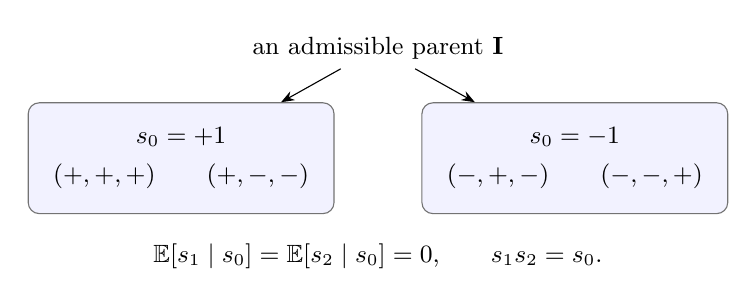
\begin{tikzpicture}[font=\small,
 box/.style={draw=black!55,rounded corners,inner sep=9pt,align=center},
 >=Stealth]
 \node (parent) at (0,1.4) {an admissible parent \(\mathbf I\)};
 \node[box,fill=blue!5] (plus) at (-2.5,0)
 {\(s_0=+1\)\\[3pt]
 \((+,+,+)\qquad(+,-,-)\)};
 \node[box,fill=blue!5] (minus) at (2.5,0)
 {\(s_0=-1\)\\[3pt]
 \((-,+,-)\qquad(-,-,+)\)};
 \draw[->] (parent) -- (plus);
 \draw[->] (parent) -- (minus);
 \node[align=center] at (0,-1.25)
 {\(\E[s_1\mid s_0]=\E[s_2\mid s_0]=0\),\qquad
   \(s_1s_2=s_0\).};
\end{tikzpicture}
\caption{The four admissible child sign triples, grouped by the
first sign. Conditional on \(s_0\), the two possibilities in its box
have equal probability. Each neighboring sign is unbiased, but their
product is fixed. The sum of the two incident-edge Grams in
\eqref{eq:child-gram} uses only these marginal averages.}
\label{fig:children}
\end{figure}


\begin{proposition}[Local energy increase]\label{prop:increase}
For \(\mathbf I\in\cA_k\), \(k\ge m+1\), define
\[
 \delta(\mathbf I)
 =\frac14\sum_{\mathbf I'\in\operatorname{ch}(\mathbf I)}
                     e(\mathbf I')-e(\mathbf I).
\]
Then \(\delta(\mathbf I)\ge0\), and
\begin{equation}\label{eq:local-control}
 \abs{\tau(\mathbf I)}
       \le\frac{10\sqrt2}{3}\,\delta(\mathbf I).
\end{equation}
\end{proposition}

\begin{proof}
We keep the parent spaces fixed and extend each child matrix by zero.
Set
\[
 C_v=(\Id+s_vD_v)^{1/2}.
\]
It is \(\sqrt2\) times the projection onto the atoms in the chosen
half. Child probability weights double, so the extended child edge
matrix is \(C_vW_vC_{v+1}\). Its row star is
\[
 R_v(s)=C_vR_v\diag(C_{v+1},C_{v-1}).
\]
In particular,
\begin{equation}\label{eq:child-gram}
 R_v(s)R_v(s)^*
 =C_v\bigl(
 W_vC_{v+1}^2W_v^*
 +W_{v-1}^*C_{v-1}^2W_{v-1}
 \bigr)C_v.
\end{equation}
Fix \(s_v\). Each neighboring sign is still uniform, so its squared
multiplier has conditional expectation \(\Id\).
Although the neighbors are correlated, \eqref{eq:child-gram} has
no product between their multipliers. Thus
\[
 \E\bigl[R_v(s)R_v(s)^*\mid s_v\bigr]
       =C_vR_vR_v^*C_v.
\]
By the convexity in Lemma~\ref{lem:hessian},
\begin{equation}\label{eq:conditional}
 \E\bigl[e_v(\mathbf I(s))\mid s_v\bigr]
       \ge\Phi(C_vR_vR_v^*C_v)
       =\Phi(T_v+s_vU_v),
 \qquad U_v=R_v^*D_vR_v.
\end{equation}
The equality compares the two Gram matrices of \(C_vR_v\):
their nonzero eigenvalues agree, even though they act on different
spaces.

Since \(D_v\) is a symmetric contraction, \(-T_v\le U_v\le T_v\).
Averaging \eqref{eq:conditional} over \(s_v=\pm1\) and applying
Corollary~\ref{cor:gap} gives
\[
 \frac14\sum_{\mathbf I'\in\operatorname{ch}(\mathbf I)}
                     e_v(\mathbf I')-e_v(\mathbf I)
       \ge\frac{1}{2\sqrt2}b_{T_v}(U_v).
\]
Summing over \(v\) proves nonnegativity of \(\delta\).
Proposition~\ref{prop:trace} now gives
\[
 \abs{\tau(\mathbf I)}
 \le\frac53\sum_v b_{T_v}(U_v)
 \le\frac{10\sqrt2}{3}\delta(\mathbf I),
\]
as asserted.
\end{proof}

\section{Summation and passage to measurable inputs}\label{sec:summation}

The local increase from Proposition~\ref{prop:increase} has the sign
needed for telescoping toward finer scales. This use of an energy
difference parallels the Bellman-function summations in
\cite[Section~2]{Kovac2011} and \cite[Lemma~2]{Kovac2012}.
We bound the total energy at each level before carrying out that sum.

\begin{lemma}[Total energy]\label{lem:total}
For the step functions of Section~\ref{sec:dyadic} and every \(k\ge m\),
set
\[
 J_k=\sum_{\mathbf I\in\cA_k}2^{2k}e(\mathbf I).
\]
Then
\begin{equation}\label{eq:total}
 0\le J_k\le2\sqrt2\sum_{v=0}^2\norm{F_v}_3^3.
\end{equation}
For \(k\ge m+1\),
\begin{equation}\label{eq:telescope}
 \sum_{\mathbf I\in\cA_k}2^{2k}\delta(\mathbf I)
       =J_{k-1}-J_k.
\end{equation}
\end{lemma}

\begin{proof}
If \(a,b\) are the Hilbert--Schmidt norms of the two edges incident
to \(v\), then
\[
 e_v(\mathbf I)
 =\tr(T_v^{3/2})
 \le(\tr T_v)^{3/2}
 =(a^2+b^2)^{3/2}
 \le\sqrt2(a^3+b^3).
\]
For an edge \(W_v\), its probability normalization gives
\begin{equation}\label{eq:edge-mass}
 \norm{W_v}_{\HS}^3
 =\left(\frac1{\abs{I_v}\abs{I_{v+1}}}
          \int_{I_v\times I_{v+1}}\abs{F_v}^2\right)^{3/2}
 \le \frac1{\abs{I_v}\abs{I_{v+1}}}
          \int_{I_v\times I_{v+1}}\abs{F_v}^3.
\end{equation}
Every edge occurs in two row stars. Also, every ordered pair of
intervals in \(\cD_k\) determines exactly one admissible third
interval, by XOR. Multiplication by \(2^{2k}=\abs{I_v}\abs{I_{v+1}}\)
and summation of \eqref{eq:edge-mass} therefore prove \eqref{eq:total}.
These sums are finite: compact support leaves finitely many nonzero
edge matrices, each belonging to one admissible triple.

Deleting the last bit of each child index shows that every admissible
child has a unique admissible parent. As
\(2^{2k}/4=2^{2(k-1)}\), the child part in the definition of
\(\delta\) sums to \(J_{k-1}\), proving \eqref{eq:telescope}.
\end{proof}

\begin{proof}[Proof of Theorem~\ref{thm:main} for step functions]
The case \(S=\varnothing\) is immediate. Otherwise set
\(k_-=\min S\), \(k_+=\max S\), and refine the common atom level,
if necessary, so that \(m\le k_--1\). By \eqref{eq:trace-integral},
Proposition~\ref{prop:increase}, and Lemma~\ref{lem:total},
\begin{align*}
 \sum_{k\in S}\sum_{\mathbf I\in\cA_k}\abs{L_{\mathbf I}(F_0,F_1,F_2)}
 &\le\frac{10\sqrt2}{3}
       \sum_{k=k_-}^{k_+}(J_{k-1}-J_k)\\
 &\le\frac{10\sqrt2}{3}J_{k_--1}
 \le\frac{40}{3}\sum_{v=0}^2\norm{F_v}_3^3.
\end{align*}
The insertion of missing scales is valid because each energy
difference is nonnegative. If every input has nonzero norm, apply
this estimate to \(F_v/\norm{F_v}_3\). Trilinearity of each local
integral gives \eqref{eq:main}, with constant \(40\).
If any norm is zero, the local integrals vanish.
\end{proof}

To pass to general inputs we need continuity of the absolute sum,
not merely continuity of the signed form. The following fixed-level
estimate provides it.

\begin{lemma}[Continuity at one scale]\label{lem:continuity}
For every \(k\in\Z\) and real \(F_v\in L^3(\R_+^2)\),
\begin{equation}\label{eq:one-scale}
 \sum_{\mathbf I\in\cA_k}\abs{L_{\mathbf I}(F_0,F_1,F_2)}
       \le\prod_{v=0}^2\norm{F_v}_3.
\end{equation}
Consequently the sequence
\((L_{\mathbf I}(F_0,F_1,F_2))_{\mathbf I\in\cA_k}\) depends
continuously on the inputs as a map from \(L^3\times L^3\times L^3\)
to \(\ell^1(\cA_k)\).
\end{lemma}

\begin{proof}
Define the nonnegative edge averages
\[
 a_v(\mathbf I)=
 \frac1{\abs{I_v}\abs{I_{v+1}}}
            \int_{I_v\times I_{v+1}}\abs{F_v}^3.
\]
H\"older's inequality on the product probability space of the three
intervals, with the Haar signs bounded by one, gives
\[
 \abs{L_{\mathbf I}(F_0,F_1,F_2)}
       \le2^{2k}\prod_{v=0}^2 a_v(\mathbf I)^{1/3}.
\]
Apply H\"older again, now to the sum over \(\cA_k\) with weight
\(2^{2k}\). The uniqueness of the third interval yields
\[
 \sum_{\mathbf I\in\cA_k}2^{2k}a_v(\mathbf I)=\norm{F_v}_3^3,
\]
proving \eqref{eq:one-scale}. These bounds also justify all integrals
and absolute sums for \(L^3\) inputs.

For two input triples \(F,G\), expand the difference of local
integrals into the three terms with inputs
\[
 (F_0-G_0,F_1,F_2),\quad
 (G_0,F_1-G_1,F_2),\quad
 (G_0,G_1,F_2-G_2).
\]
Estimate each term by \eqref{eq:one-scale}. If \(G_v\to F_v\) in
\(L^3\), the sum of these three product bounds tends to zero.
This is the asserted \(\ell^1\) continuity.
\end{proof}

\begin{proof}[Completion of Theorem~\ref{thm:main}]
Bounded compactly supported dyadic step functions are dense in
\(L^3(\R_+^2)\). To see this, first approximate an \(L^3\) function by
a continuous compactly supported function, then take its averages on
sufficiently small dyadic squares. Uniform continuity and a common
bounded support give convergence in \(L^3\).

For arbitrary real \(F_v\in L^3\), choose such step functions
\(F_v^{(n)}\to F_v\) in \(L^3\). Assuming \(S\ne\varnothing\),
refine their common atom levels, without changing the functions, to
satisfy \(m_n\le\min S-1\). Apply the step-function estimate to these
inputs. Lemma~\ref{lem:continuity}, summed over the fixed finite set
\(S\), gives convergence of their local integrals in \(\ell^1\).
The inequality \(\abs{\abs a-\abs b}\le\abs{a-b}\) permits passage to
the absolute sum in \eqref{eq:main}, and norm convergence handles its
right-hand side. This proves the theorem and its stated extension
to real \(L^3\) inputs. The case \(S=\varnothing\) remains immediate.

For any coefficients
\(\abs{\epsilon_{\mathbf I}}\le1\), the triangle inequality gives
the corresponding bound for
\[
 \sum_{k\in S}\sum_{\mathbf I\in\cA_k}
 \epsilon_{\mathbf I}L_{\mathbf I}(F_0,F_1,F_2).
 \qedhere
\]
\end{proof}

\bibliographystyle{plain}
\bibliography{references}
\end{document}
